\chapter{Stand van zaken}
\label{ch:stand-van-zaken}

% Tip: Begin elk hoofdstuk met een paragraaf inleiding die beschrijft hoe
% dit hoofdstuk past binnen het geheel van de bachelorproef. Geef in het
% bijzonder aan wat de link is met het vorige en volgende hoofdstuk.

% Pas na deze inleidende paragraaf komt de eerste sectiehoofding.

In dit hoofdstuk wordt de stand van zaken besproken wat tabeltransformatie van afbeeldingen betreft. Er wordt besproken wat tabulair data is, waarom tabellen belangrijk zijn in de huidige informatiewereld, wat er bedoeld wordt met tabeldetectie en structuuranalyse, waar de uitdagingen hierbij zich bevinden en tenslotte wordt er in detail de verschillende technieken besproken die ontwikkeld werden om tabellen te kunnen detecteren en analyseren, met hun voor- en nadelen.

\section{Tabulair data}
\label{sec:tabulair-data}

\subsection{Definitie}
\label{subsec:definitie-tabulair-data}

Zoals \textcite{Zanibbi2003} het aangeeft, is een tabel een vorm van visualiatie dat men gebruikt om ermee data op te zoeken en te vergelijken. Meer specifiek geeft, volgens \textcite{Zanibbi2003}, een tabel indexeringschema's weer voor relaties. Een relatie heeft een verzameling van $\eta$ \glspl{tupel}, die de domeinen of dimensies van de relatie genoemd worden.

De dimensies kunnen d.m.v. verschillende combinaties van rijen en kolommen opgesteld worden, waardoor verschillende tabelopstellingen exact dezelfde informatie op verschillenden manieren kunnne weergeven. Dit kan gedemonstreerd worden a.d.h.v. de volgende twee figuren.

\begin{figure}[H]
    \centering
    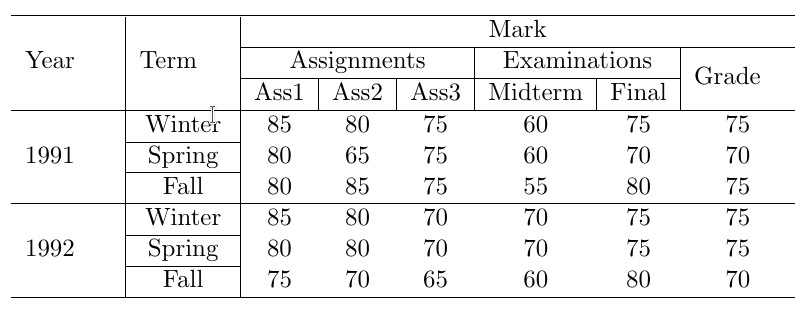
\includegraphics[width=0.8\textwidth]{img/tabel_verschillende_opstelling_dezelfde_data_1.png}
    \caption{Een tabel van evaluaties. Het geeft dezelfde informatie weer als tabelfiguur \ref{fig:tabel_verschillende_opstelling_dezelfde_data_2}. Bron: \cite{Long2010}}
    \label{fig:tabel_verschillende_opstelling_dezelfde_data_1}
\end{figure}

\begin{figure}[H]
    \centering
    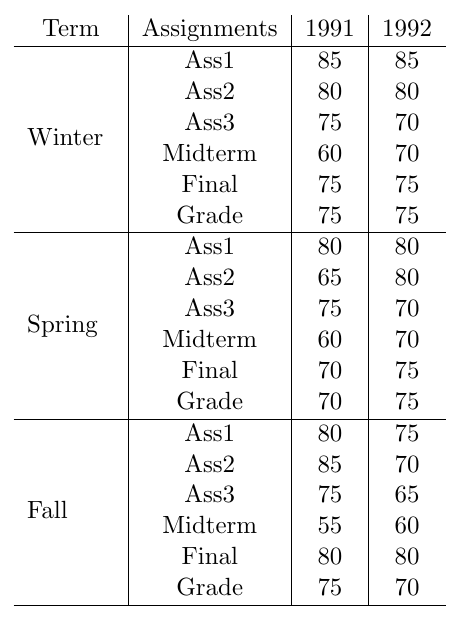
\includegraphics[width=0.5\textwidth]{img/tabel_verschillende_opstelling_dezelfde_data_2.png}
    \caption{Een tabel van evaluaties. Het geeft dezelfde informatie weer als tabelfiguur \ref{fig:tabel_verschillende_opstelling_dezelfde_data_1}. Bron: \cite{Long2010}}
    \label{fig:tabel_verschillende_opstelling_dezelfde_data_2}
\end{figure}

Hoewel beide tabellen identiek zijn wat informatieinhoud betreft, kan duidelijk gemerkt worden dat tabelfiguur \ref{fig:tabel_verschillende_opstelling_dezelfde_data_1} de evaluaties duidelijker weergeeft. Meestal wordt een combinatie van rijen en kolommen zodanig gekozen zodat de data van de tabel zo eenvoudig en snel mogelijk gelezen en geïnterpreteerd kan worden. Ook kunnen verschillende lettertypes, kleuren en lettergroottes gebruikt worden om de leesbaarheid te vergroten.

\subsection{Anatomie}
\label{subsec:anatomie}

\raggedbottom

Volgens \textcite{Wang1996} is een tabel, door \textit{stub scheiding} en \textit{boxhead scheiding}, verdeeld in vier hoofdregio's die in onderstaande figuur \ref{fig:tabel_anatomie} merkbaar zijn. De regio linksbeneden die de rijhoofdingen bevat en de regio rechtsboven die de kolomhoofdingen bevat, worden respectievelijk de \textit{stub} en de \textit{boxhead} genoemd. De regio linksboven, die de categorieën in de \textit{stub} inhouden is gekend als de \textit{stub head} en de \textit{body} tenslotte, is de regio rechts van de \textit{sub} en onder de \textit{boxhead} die de tabeldata-elementen bevat. De snijpunt van een rij en een kolom wordt een \textit{cel} genoemd; en een rechthoekig verzameling van \textit{cellen} is gekend als een \textit{block}.

\begin{figure}[H]
    \centering
    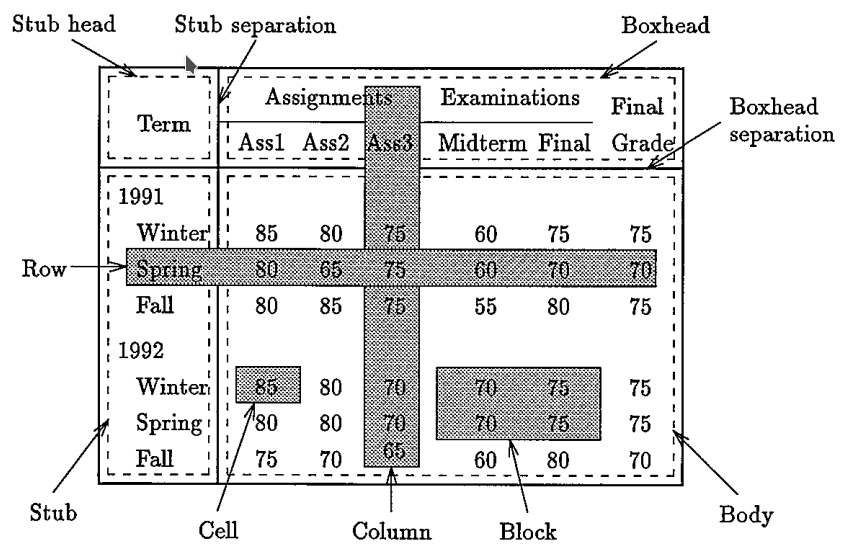
\includegraphics[width=0.8\textwidth]{img/tabel_anatomie.png}
    \caption{De anatomie van de structurele rij-kolomvoorstelling van een tabel. Bron: \cite{Wang1996}}
    \label{fig:tabel_anatomie}
\end{figure}

Zoals men in figuur \ref{fig:tabel_anatomie} kan zien, kunnen multidimensionele relaties in een twee dimensionele tabel gepresenteerd worden door meer dan één categorie te associeren met de \textit{boxhead} en/of met de \textit{stub}. Zo worden hier de rijhoofdingen niet enkel met één hoofdcategorie ``Term`` maar eveneens met meerdere subcategorieën, ``1991`` en ``1992`` geassocieerd. Analoog zijn de kolomhoofdingen gekoppeld aan drie categorieën, namelijk ``Assignments``, ``Examinations`` en ``Finals``.

\subsection{Functie}
\label{subsec:functie}

Als vermeld door \textcite{Shahzad2019}, worden tabellen veelal gebruikt voor het gestructureerd vertonen van essentiële informatie in documenten. Ze worden gebruikt in boeken, artikelen, onderzoekspapers, en verschillende andere soorten media. In sectoren zoals de financiële en de administratieve sectoren wordt data veelal in tabelvorm geformuleerd omdat tabellen, volgens \textcite{Coueasnon2014}, veel informatie voorstellen op een beknopte manier waardoor het begrijpbaar blijft voor de lezer; ze laten ook zo toe de belangrijke delen te benadrukken. 

\subsection{Creatie en representatie}
\label{subsec:creatie-en-representatie}

Doorheen de tijd werden verschillende software applicaties ontwikkeld om digitaal tabulair data aan te maken, te beheren en voor te stellen. Een veelgebruikte software voor tabelcompositie is Microsoft Excel. Het is, zoals \textcite{Wang1996} het vermeldt, een complexe rekenbladprogramma waarbij tabulair data in een werkblad, in een twee dimensionele rooster die a.d.h.v. rij en kolomindexes geadresseerd kan worden, geplaatst wordt.

Een andere bekend software voor het creëren van tabellen is \LaTeX. Het is een systeem voor het zetten van documenten. \textcite{Wang1996} geeft aan dat tabellen in \LaTeX\ gespecifieerd kunnen worden met de ``tabular``- en de ``array``-omgeving. De eerste omgeving wordt meestal gebruikt voor tekstuele tabeldata, de tweede voor wiskundige uitdrukkingen.

Voor de voorstelling van tabellen op het internet, m.a.w. op internetbrowsers, wordt de opmaaktaal HTML gebruikt. Door middel van de ``table``-, ``tr``-, ``th``- en ``td``-tags kunnen tabellen gemaakt en voorgesteld worden.

\section{Tabeltransformatie}
\label{sec:tabel-transformatie}

Verschillende technieken om tabeltransformatie werden reeds ontwikkeld. Echter blijft een algemeen toepasbare oplossing een moeilijk uitdaging, en dit voor diverse redenen.

\begin{itemize}
    \item Tabellen bezitten uiteenlopende layouts en designs, zonder enige standaardisatie
          \autocite{Kasar2014}
    \item Verschillende tabellayouts hebben verschillende features \autocite{Kasar2014}
    \item De typisch kleine inter-klasse variantie tussen tabellen, figuren en grafieken vermoeilijkt
          de detectie van tabellen; de kleine variantie is verantwoordelijk voor de hoge hoeveelheid
          valse positieven bij tabeldetectie \autocite{Embley2006}
  \end{itemize}

\textcite{Kasar2014} beschreeft tabeltransformatie als een proces bestaand uit voornamelijk twee subprocessen: tabeldetectie en tabelstructuuranalyse. 

Met tabeldetectie worden eerst regio's in een bepaalde document geïdentificeerd die overeenkomen met tabellen. Vervolgens wordt tabelstructuuranalyse toegepast om relationele informatie te extraheren van de geïdentificeerde tabelregio's om de logische structuur van de tabellen te achterhalen, zoals bijvoorbeeld de rijhoofdingen, kolommhoofdingen, cellen en meer.

\subsection{Tabeldetectie}
\label{subsec:tabel-detectie}

Tabeldetectietechnieken kan men, kijkend naar de stand van zaken, opdelen in twee klassen: klassieke, op regelgebaseerde algoritmen enerzijds en de recentere, opkomende algoritmen die gebruik maken van machinaal leertechnieken.

\subsubsection{Regelgebaseerde technieken}

\textcite{Watanabe1991} was de auteur van één van de vroegste werken om tabellen te identificeren. De basis voor de tabelidentificatie hier is de identificatie van individuele blokken, ingesloten door horizontale en verticale lijnsegmenten. Eerst worden lijnsegmenten gedetecteerd en hiermee wordt vervolgens de positie van hoekpunten, gevormd door deze lijne, bepaald. Hierna wordt a.d.h.v. de poositie van deze hoekpunten individuele blokken geïdentificeerd. De relatie tussen de verschillende blokken wordt uiteindelijk in globale en individuele boomstructuren gebruikt om te beslissen of het over een tabel gaat of niet.

Het jaar daarop stelde \textcite{Laurentini1992} een methode voor waarbij tekstregio's op een bottom-up manier gedetecteerd worden. De gedetecteerde karakters worden samengebracht tot woorden en deze woorden worden op hun beurt aan elkaar samengevoegd tot tekstblokken. Ook worden de scheidingslijnen gedeteceerd. Voor elke tekstblok wordt diens positie vergeleken met de scheidingslijnen, om te bepalen of het tot een bepaalde tabel behoort.

TINTIN werd door \textcite{Pyreddy1997} voorgesteld, om tabellen te detecteren. Hun algoritme steunt voor de analyse op de extra PDF-metadata van de PDF-documenten.

Enkele jaren later werd het systeem T-Recs, door \textcite{Kieninger2001}, voorgesteld. Het systeem vormt rechthoeken (bounding boxes) voor woorden in het tabel en op een bottom-up manier worden deze bounding boxes gegroepeerd volgens hun logische eenheden. 

\subsubsection{Datagedreven technieken}

Datagedreven technieken vereisen veel data om nauwkeurig te kunnen werken. Indien het om gesuperviseerde machinale leertechnieken gaat, is er daarbij nog ground truth labeling van de tabeldatasets nodig, wat een tijdrovend proces is. \textcite{Wangt2001} ontwikkelde een galabelde dataset generator die op basis van één gelabelde tabel, met bijhorende metadata, automatisch, mits kleinde aanpassingen, datasets van gelabelde tabelafbeeldingen genereert en dus de ground truth labeling proces automatiseert. Deze tool zou zeer handig geweest zijn voor modeltraining van datagedreven algoritmen en voor algoritme-evaluaties. \citeauthor{Wangt2001} werd voor gecontaceerd om deze tool beschikbaar te maken maar helaas is de software niet meer ter beschikking.

Objectdetectie bij afbeeldingen d.m.v. machinale leertechnieken is sinds enkele tiental jaren een populair onderzoeksonderwerp geworden. De traditionele pipeline voor objectdetectie bestaat uit een feature extraheerder (feature extractor), gevolgd door een classificatiesysteem.

\textcite{Cesarini2002} was één van de eersten die geprobeerd heeft machinale leertechnieken te gebruiken voor tabeldetectie. Hierbij wordt, door de besproken methode Tabfinder, de document omgezet in een MXY-boomvoorstelling en wordt er gezocht naar blokken omgeven door horizontale of verticale lijnen; dit gebeurt recursief. Indien deze verticale of horizontale lijnen gevonden zijn, dan bevat het document mogelijks een tabel. Om de veronderstelling te verifiëren, wordt er in diepere niveaus van de boom gezocht naar lijnen die loodrecht staan op de reeds gedetecteerde lijnen. Indien deze lijnen daarbovenop gevonden zijn, dan kan er met zekerheid vastgesteld worden dat het om een tabel in het document gaat. Na de boomanalyse worden vervolgens subtabellen behorend tot dezeflde tabel samengevoegd.

In een paper introduceert \textcite{Mandal2006} een simpele maar efficiënte algoritme om tabellen te identificeren. De algoritme steunt namelijk op de observatie dat de hoeveelheid witruimte tussen elementen van verschillende kolommen significant groter is dan de witruimte tussen woorden in paragrafen.

\textcite{Silva2009} heeft eveneens een data-gedreven model voorgesteld, gebruikmakend van Hidden Markow Modellen en PDF-documenten. De tekst van de PDF-documenten worden eerst omgezet in ASCII-karakters, en hierna verwerken de Hidden Markdov Modellen de waarschijnlijkheidsdistributies van de samenhang van de verschillende opeenvolgende ASCII-karakters. De modellen houden voor elke horizontale lijn ook bij of het deel uitmaakt van een tabel, of niet.

Een SVM-classificatiesysteem, steunend op enkele manueel geselecteerde dimensiefeatures van de horizontale en verticale scheidingslijnen, werd door \textcite{Kasar2013} gepresenteerd. Om de donkere, dunne en lijnachtige structuren, die als scheidingslijnen van een tabel beschouwd worden, goed te kunnen detecteren, wordt de inputafbeelding eerst verzacht met een Gaussiaanse filter. Vervolgens worden op de input enkele top-hat-transformaties toegepast. Uiteindelijk wordt voor elke groep van kruising van horizontale en verticale lijnen een SVM-classifier met 26 lijnfeatures gebruikt om te bepalen of de regio deel uitmaakt van een tabel.

\textcite{Fan2015} gebruikte zowel een niet-gesuperviseerde leermodel als tekstuele informatie van een bepaalde zone voor de detectie van tabellen. De gebruikte niet-gesuperviseerde leermodel bestaat uit een ensemble van generatieve en distriminatieve modellen.

In hetzelfde jaar presenteerde \textcite{Tran2015} een methode die zich baseert op de ruimtelijke ordening van uitgehaalde tekstblokken en op ROI's. In tegenstelling tot verschillende andere traditionele algoritmen, is hun voorstel direct bruikbaar op afbeeldingen van gescande documnenten.

Eén van de eerste pogingen om deep learning toe te passen, werd gerealiseerd door \textcite{Hao2016}. Kandidaattabellen worden geselecteerd op basis van scheidingslijnfeatures. Hierna worden deze Kandidaattabellen verwerkt door een CNN. Uiteindelijk vindt de klassificatie ``tabel`` of ``geen tabel`` plaats.

\textcite{Rashid2017} gebruikte een bottom-up algoritme waarbij voor elk woord een feature-vector werd aangemaakt. Elke feature-vector bevat features zoals de dimensies van het woord, de afstand tot de andere woorden in de nabijheid, de hoeveelheid witruimte, etc. Deze feature-vectors werden uiteindelijk gebruikt om een AutoMLP-klassificatiessysteem te trainen.

Een andere deep learning techniek, gebaseerd op de Faster R-CNN-architectuur werd voorgesteld door \textcite{Gilani2017}. Normaliter worden pixelwaarden als input gebruikt, voor een convolutionele neurale netwerk. Bij dit onderzoek is dat niet het geval. In plaats van pixelwaarden wordt de witruimte tussen tekstblokken als input verwerkt, aangezien bij tabellen witruimte tussen tekstblokken een bepaalde patroon bevat die door het model gedetecteerd wordt.

Faster R-CNN is een poopulaire modelkeuze geworden door de hoge nauwkeurigheid dat het aanbiedt bij objectdetectie in verschillende domeinen. Het bestaat, zoals meegedeeld door \textcite{Shahzad2019}, uit twee processen die sequentieel uitgevoerd worden. Het eerste proces is Region Proposal Network (RPN) dat kandidaaatregio's voor de detectienetwerk identificeert. Het tweede proces is de klassificatiesysteem die a.d.h.v. de detectienetwerk voor elke kandidaatregio beslit of het als een tabel beschouwd kan worden of niet. De RPN-module van Faster R-CNN biedt hogere performantie dan de selectieve zoekproces (selective search) van Fast R-CNN, de voorganger van Faster R-CNN.

\textcite{Siddiqui2018} introduceerde een incrementele architectuurverbetering, door Faster R-CNN te combineren met een vervormbare (deformable) CNN. De RestNet-101-model werd gebruikt voor transfer learning, aangezien er niet voldoende gelabelde data beschikbaar was. De reden waarom gebruik gemaakt werd van een vervormbare CNN i.p.v. een klassieke CNN is dat de klassieke CNN een vaste receptieve veld heeft (fixed receptive field), wat niet gewenst is door de verschillende dimensies en transformaties zoals verdraaing, vergroting, verschuiving en meer dat tabellen kunnen hebben. Een vervormbare CNN kan zijn receptieve veld aanpassen aan de inputdata, hierdoor is het te gebruiken op elk soort tabel, ongeacht de layout ervan.

\subsection{Tabelstructuuranalyse}
\label{subsec:tabel-structuur-analyse}

\subsection{End-to-end-systemen}
\label{subssec:end-to-end-systemen}
